\begin{figure}[H]
	\centering
	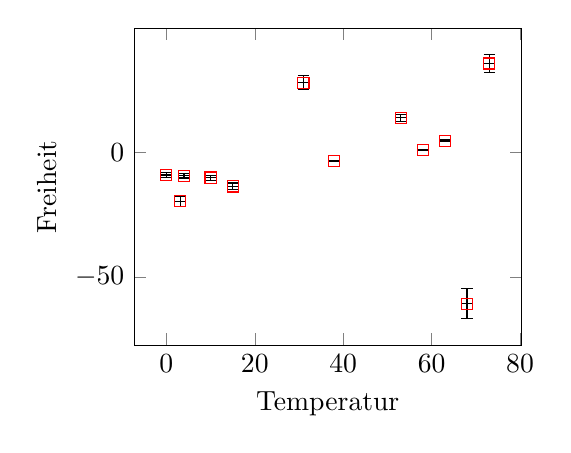
\begin{tikzpicture}
		\pgfplotsset{width=6.5cm,compat=1.3,legend style={font=\footnotesize}}
		\begin{axis}[xlabel={Temperatur},ylabel={Freiheit},legend cell align=left,legend pos=north west]
		\addplot+[only marks,color=red,mark=square,error bars/.cd,x dir=both,x explicit,y dir=both,y explicit,error bar style={color=black}] table[x=X,y=Y,x error=xerror,y error=yerror,row sep=\\]{
			X	Y	xerror	yerror	\\
			3.141592653589793	-19.587152221267605	0	-1.9587152221267605 (1/())	\\
			73	35.61118695932225	0	3.5611186959322247 (1/())	\\
			68	-60.65178959028931	0	-6.065178959028931 (1/())	\\
			63	4.697996134713314	0	0.4697996134713314 (1/())	\\
			58	0.8484052762734677	0	0.08484052762734678 (1/())	\\
			53	13.795175511942787	0	1.3795175511942788 (1/())	\\
			38	-3.4407061579130485	0	-0.3440706157913049 (1/())	\\
			31	27.950236316457676	0	2.7950236316457677 (1/())	\\
			15	-13.68049659008453	0	-1.3680496590084532 (1/())	\\
			10	-10.126471807847185	0	-1.0126471807847186 (1/())	\\
			4	-9.352740465879492	0	-0.9352740465879492 (1/())	\\
			0	-9.080536481984176	0	-0.9080536481984176 (1/())	\\
		};		% \addlegendentry{Messpunkte Datensatz 0}
		\end{axis}
		\end{tikzpicture}
	\caption{$f(T)$}
	\label{fig:FreiheitTemperatur}
\end{figure}